% -*- coding: utf-8 -*-
\documentclass{article}
\usepackage{listings}
\usepackage{ctex}
\usepackage{graphicx}
\usepackage[a4paper, body={18cm,22cm}]{geometry}
\usepackage{amsmath,amssymb,amstext,wasysym,enumerate,graphicx}
\usepackage{float,abstract,booktabs,indentfirst,amsmath}
\usepackage{array}
\usepackage{booktabs} %调整表格线与上下内容的间隔
\usepackage{multirow}
\usepackage{url}
\usepackage{diagbox}
\renewcommand\arraystretch{1.4}
\usepackage{indentfirst}
\usepackage{booktabs}
\usepackage[table,xcdraw]{xcolor}
\setlength{\parindent}{2em}
\usepackage[colorlinks,linkcolor=black]{hyperref}
\usepackage{listings}
\usepackage{xcolor}

\lstset{
	numbers=left, 
	numberstyle= \tiny, 
	keywordstyle= \color{ blue!70},
	commentstyle= \color{red!50!green!50!blue!50}, 
	frame=shadowbox, % 阴影效果
	rulesepcolor= \color{ red!20!green!20!blue!20} ,
	escapeinside=``, % 英文分号中可写入中文
	xleftmargin=2em,xrightmargin=2em, aboveskip=1em,
	basicstyle=\footnotesize,
	framexleftmargin=2em
} 


\geometry{left=2.8cm,right=2.2cm,top=2.5cm,bottom=2.5cm}
%\geometry{left=3.18cm,right=3.18cm,top=2.54cm,bottom=2.54cm}

\graphicspath{{figures/}}

\title{\heiti 时间序列大作业}

\begin{document}
	\maketitle
	%\tableofcontents
	
	\begin{center}
		%\LARGE{{\textbf{\heiti 实验一 远程过程调用中间件及数据访问中间件}}}
		%\newline
		%\newline
		%\date{2019年4月2日}
		\begin{table}[H]
			\centering
			\begin{tabular}{p{3cm}p{4cm}<{\centering}p{3cm}p{4cm}<{\centering}}
				班\quad 级: & 1907031 & 学\qquad 号:   & 19070300002 \\ \cline{2-2} \cline{4-4} 
				姓\quad 名: & 徐文韬       & 指导老师: & 王红军       \\ \cline{2-2} \cline{4-4} 
			\end{tabular}
		\end{table}
	\end{center}
	


	

	

\begin{abstract}
	\zihao{-5}
		本文尝对俄乌战争中的防空炮损坏数量进行建模分析。
	\begin{enumerate}

	
	\item 首先,我们观测时间序列,这是一个明显不平稳的时间序列。通过二次差分来使得时间序列平稳化。
	
	\item 然后,我们尝试对时间序列进行ARIMA模型建模。我们通过观察ACF,PACF以及EACF图来确定模型的阶数,并借助AUTO.ARIMA函数来快速计算各个阶数组合下的AIC值来辅助我们的阶数确定。最后,我们将模型确定为ARIMA(0,2,1)模型。
	
	\item  接着,我们对模型进行模型诊断。我们通过观察残差的ACF和计算LJUNG-BOX统计量,认为残差是符合独立性假设的。接着我们观察残差的QQ图,发现发现大部分点都符合正态分布,但是有四个异常点发生了显著的偏移现象。
	
	\item 最后,我们单独分析了这四个点(2/28,3/4,3/16,4/12),发现在这四天左右发生了大规模空军的军事活动。这些特别的军事战术决策导致的异常现象是我们无法从防空炮自身的时间序列中挖掘到的。因此,我们提出了从飞机损失数量等时序中提取数据构造干预函数,从而对ARIMA模型进行修正的意见。
    \end{enumerate}
	\vspace{5pt}
	\textbf{Keywords}: ARIMA; 差分; LJUNG-BOX;  模型诊断; 干预函数
\end{abstract}

	
\tableofcontents

	\newpage
	
	\section{模型准备}
	
	
	让我们首先来仔细观察俄乌战争中,防空炮损失数量的时间序列图。
	
	
			\begin{figure}[h]
				\centering
				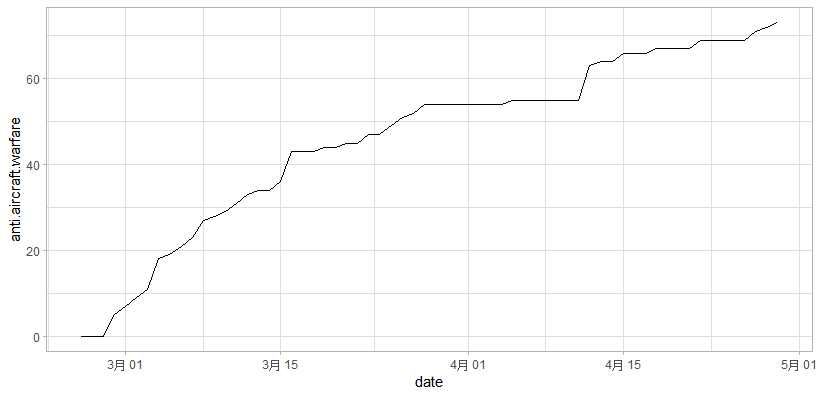
\includegraphics[width=.9\textwidth]{Rplot01.png}
				\caption{高射炮损失数量时间序列图}
			\end{figure}
	
	显然的,这个时间序列明显呈现上升趋势,所以它的均值一定不符合平稳性的要求。其次,时间序列在诸如3.16,4.11日等时间节点就陡然增加的情况,这是我们在后面的模型建立与诊断需要注意的。(数据来自\url{https://www.kaggle.com/datasets/piterfm/2022-ukraine-russian-war})
	
	
	\section{ARIMA模型建立}
	
	\subsection{平稳化}
	
	首先,正如模型准备中提到的,这个时间序列是不平稳的。它呈现上升趋势,因此我们尝试通过差分的手段将它平稳化:
	


    值得注意的是,一次差分后得到的时间数列会比原序列减少一个数据。

	\begin{figure}[H]
	\centering
	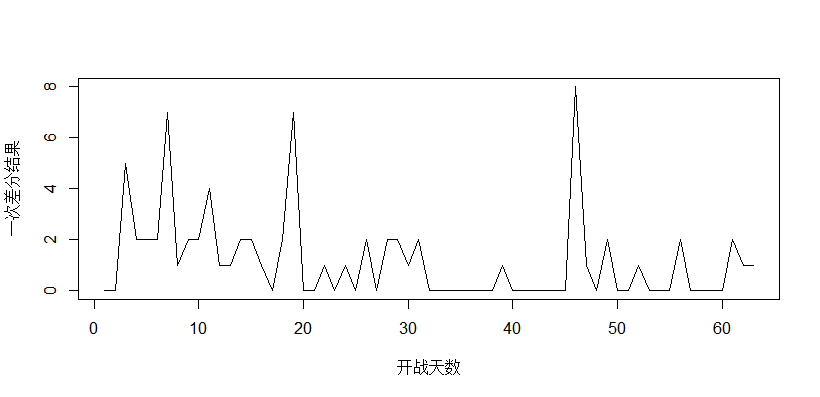
\includegraphics[width=.9\textwidth]{Rplot02.png}
	\caption{一次差分序列}
    \end{figure}
	

	我们看到经过一次差分后的时序图仍然呈现非平稳的状态:数据集中在0的上方浮动。
	
	因此,我们对时间序列进行二次差分。
	
	\begin{equation}
	\nabla^{2}Y_t=\nabla Y_t-\nabla Y_{t-1}
	\end{equation}
	
	
	\begin{figure}[H]
		\centering
		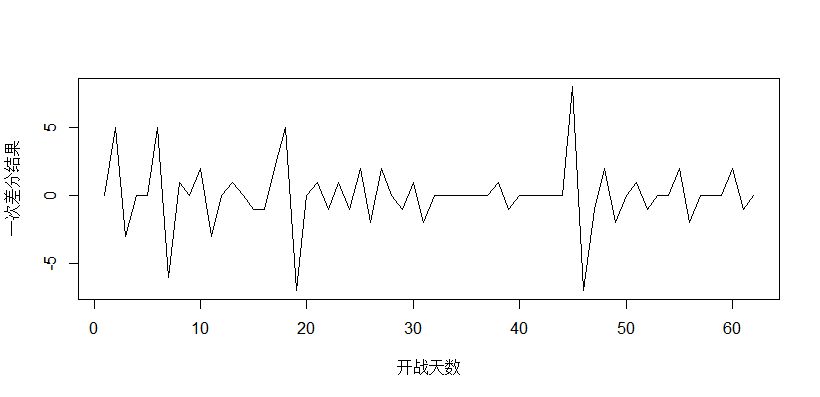
\includegraphics[width=.9\textwidth]{Rplot03.png}
		\caption{二次差分序列}
	\end{figure}
	
	经过二次差分后,我们可以看到此时的时间序列图已经呈现在0附近上下波动的状态。此时,我们认为平稳模型是恰当的。
	
	\subsection{模型介数选择}
	
	接下来,对于ARMA模型:
	\begin{equation}
		Y_t=\phi _1Y_{t-1}+\cdots +\phi _pY_{t-p}+e_t-\cdots -\theta _qe_{t-q}
	\end{equation}
	
	
	我们尝试确定它的阶数p,q,我们可以根据ACF,PACF和EACF图来进行抉择。
	
	我们首先来看ACF图。
	
	
		\begin{figure}[H]
		\centering
		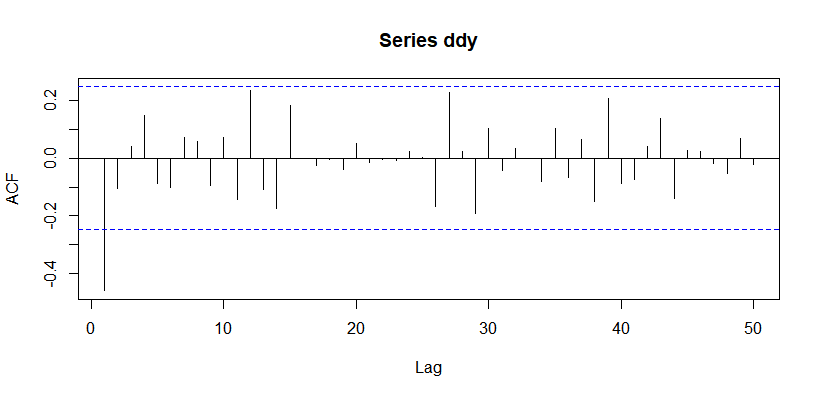
\includegraphics[width=.9\textwidth]{Rplot04.png}
		\caption{ACF图}
	\end{figure}

	当我们使用简单标准误差作为临界值时,从ACF图上我们可以看到,经过两次差分后的时间序列的自相关系数值,从滞后一节开始都都在临界范围内,可以认为是0。
	
	当然,他们在一定程度上也呈现阻尼震荡的趋势。然而一阶处的自相关系数显著的不为0,在整体上呈现出与MA(1)模型相似的一阶截尾的状态。
	
	
	接着,我们来看它的PACF图。
	
		\begin{figure}[h]
		\centering
		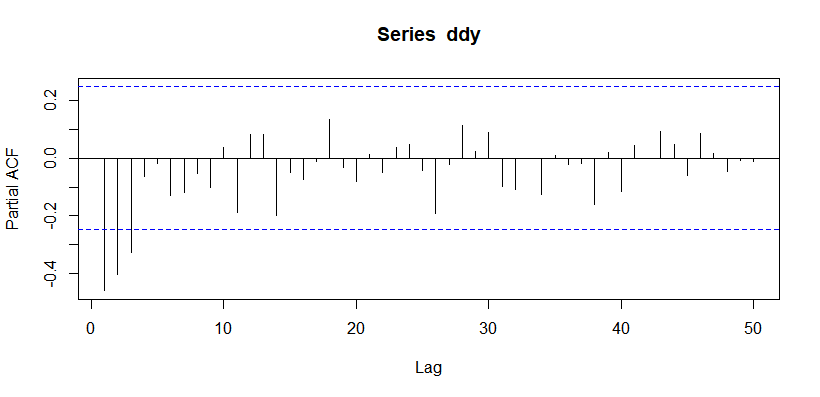
\includegraphics[width=.9\textwidth]{Rplot05.png}
		\caption{PACF图}
	\end{figure}
	
	从PACF图上,我们可以看出PACF值呈现递减趋势,随着滞后介数的增加,快速衰减至0(可以看到,在三阶滞后的PACF值已经处于临界范围内)
	
	这也是符合MA(1)模型的特点。
	
	接下来,我们通过参考EACF图来辅助判断。
	
		\begin{figure}[h]
		\centering
		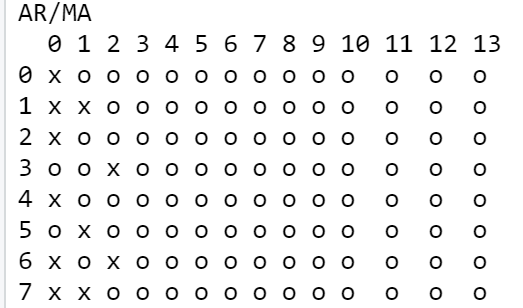
\includegraphics[width=.9\textwidth]{Rplot06.png}
		\caption{EACF图}
	\end{figure}
	
	从图上我们可以明显的看出,EACF图也建议我们对两次差分后的时间序列建立一个MA(1)模型。
	
	
	当然,我们也可以通过TSA包中的auto.arima模型对arima(p,d,q)的各种阶数的组合的情况进行汇总。
	
	
		\begin{figure}[h]
		\centering
		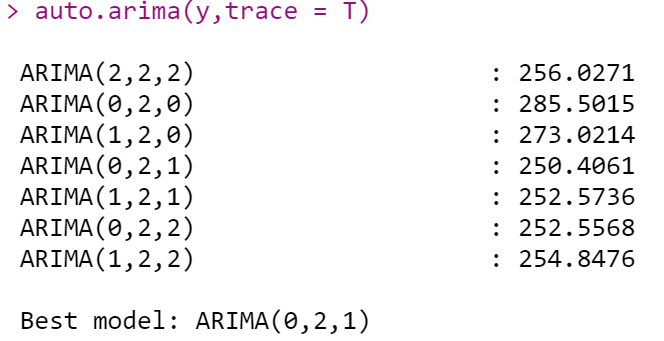
\includegraphics[width=.9\textwidth]{Rplot07.png}
		\caption{各种阶数组合}
	\end{figure}
	可以看到,以AIC值为标准,在众多阶数组合中,MA(1)模型具有最小的AIC值。同时,MA(1)模型也符合用尽量简洁的模型描述数据这一原则。
	
	
	\subsection{参数估计与拟合}
	
	由上文所述,我们欲建立一个MA(1)模型。那么对于MA(1)模型的参数估计,矩估计是不合适。因此我们尝试使用最小二乘估计和极大似然估计。
	我们使用TSA包中的ARIMA函数来计算这个过程。
	
	\begin{table}[H]
		\centering
		\caption{\textbf{MA(1)模型参数估计}} 
		\begin{tabular}{llll}
			\toprule
			& 条件SS估计  & 无条件SS估计 & 极大似然估计  \\  \hline
			估计值  & -0.8453 & -0.9080 & -0.9080 \\
			s.e. & 0.0773  & 0.0531  & 0.0531 \\ \bottomrule
		\end{tabular}
	\end{table}
	
	我们可以看到,三种估计之间相差都不大。我们不妨选择极大似然估计作为估计值。
	因此我们最后建立的是参数$
	\theta 
	$
	为:-0.908 的ARIMA(0,1,1)模型。
	
	\section{模型诊断}
	
	
	现在我们来进行模型诊断。
	首先,我们来计算残差:
	\begin{equation}
		\text{残差=实际值-预测值}
	\end{equation}
	
	按照我们所做的假设,残差应该近似于白噪声的性质。
	

	
	\begin{figure}[h]
		\centering
		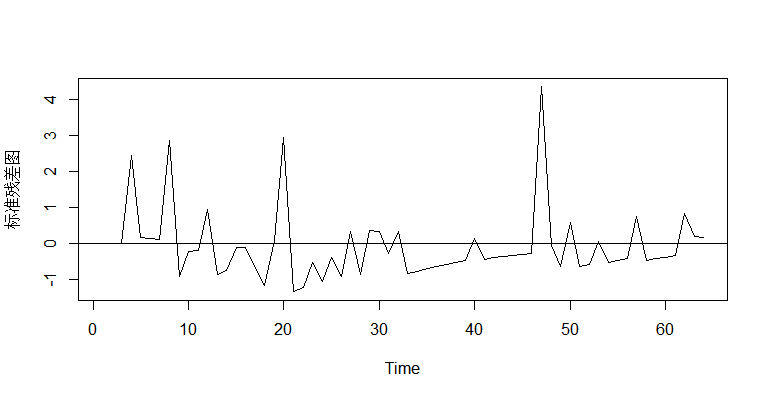
\includegraphics[width=.9\textwidth]{Rplot09.png}
		\caption{标准残差图}
	\end{figure}
	
	
	从图中我们可以看出,整个残差序列有些奇怪。在四个点(开战后第4,8,20,47天)明显的接近或超过3,这在标准正态分布中是不正常的。
	
	接着我们来残差的自相关图:
	
	
		\begin{figure}[h]
		\centering
		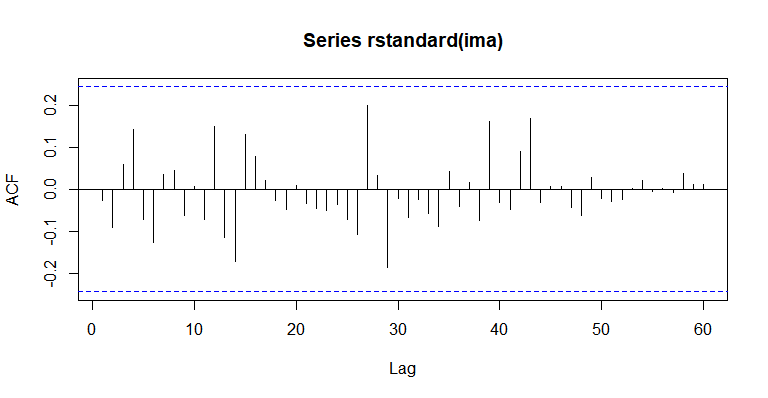
\includegraphics[width=.9\textwidth]{Rplot08.png}
		\caption{残差的ACF图}
	\end{figure}
	
	
	在ACF图中我们可以明显的看出滞后各个阶数的残差都明显的小于临界值。于是我们有理由相信这是独立的。
	
	当然,除了观察各个单独的滞后处的残差的相关系数,将这些相关系数的值作为一个组来进行检验也是有用的。我们使用LJUNG-BOX统计量:
	
	\begin{equation}
	Q_*=n\left( n+1 \right) \left( \frac{\widehat{r}_{1}^{2}}{n-1}+\cdots +\frac{\widehat{r}_{K}^{2}}{n-K} \right) 
	\end{equation}
	
	在原假设为独立分布下,有限样本的$Q_*$的分布可以参阅LJUNG和BOX(1978)以及DAVIES,TRIGGS和NEWBOLD(1977)。我们使TSA中的tsdiag函数来计算各个K值时的$p$值。
	
		\begin{figure}[h]
		\centering
		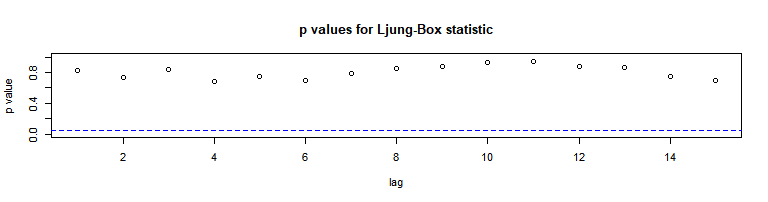
\includegraphics[width=.9\textwidth]{Rplot10.png}
		\caption{LJUNG-BOX统计量的P值}
	\end{figure}
	
	显然,我们无法拒绝误差项的独立性。
	
	但是,我们不能忽略在图8中发现的四个异常值,我们画出残差的QQ图:
	
	
		\begin{figure}[H]
		\centering
		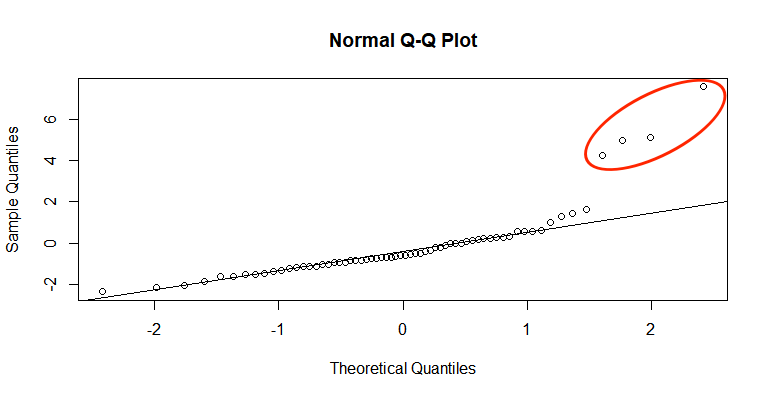
\includegraphics[width=.9\textwidth]{Rplot11.png}
		\caption{残差的QQ图}
	\end{figure}
	
	我们可以看出这四个点发生了明显的偏离现象。
	
	因此,我们的时间序列模型虽然在大部分点都取得了不错的效果,但是在某些个别点上仍然有一些值得进一步思考的地方。
	
	
	\section{问题分析与模型改进}
	
	
	正如我们在上文中提到的,有四个点明显不符合我们残差为白噪声的假设:他们分别发生在开战后第4,8,20,47天,即(2/28,3/4,3/16,4/12)
	我们来观察俄乌战争中的飞机(不包含无人机)损失数:
	
		\begin{figure}[H]
		\centering
		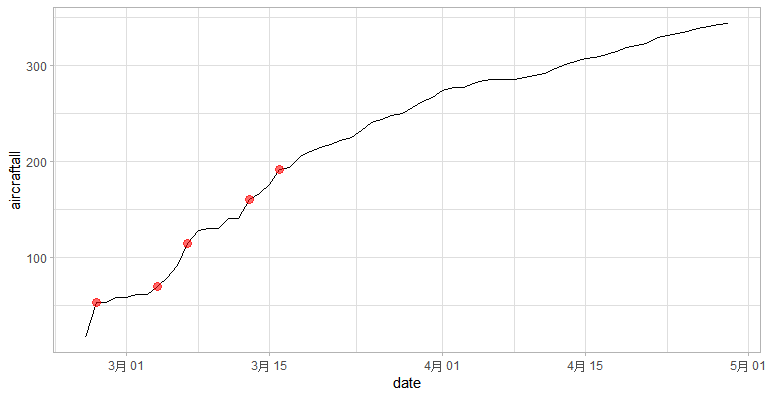
\includegraphics[width=.9\textwidth]{Rplot12.png}
		\caption{飞机损失数}
	\end{figure}
	在图12中,我们可以看到在2/28,3/4,3/16 这几天左右,出现了飞机损失数陡增的现象。
	而在4/12号的战报上,我们可以看到俄罗斯国防部发言人伊戈尔在记者会上说:俄军使用“口径”海基高精度导弹摧毁了4套S-300防空导弹系统,在第聂伯罗郊区摧毁了欧洲提供的S-300防空导弹系统。
	
	所以,我们有理由猜测在这几个天发生的残差值异常是由于军事冲突的突然升级,一些空军战术决策导致的。
	
	而这种因素,我们是很难从防空炮损失数量自身的时间序列中挖掘到的,我们需要通过对其他的时间序列,如飞机损失数,整个冲突激烈程度等时间序列中提取相关因素,来建立起一个干预函数$m_t$
	
	从而对我们的时间序列做出修正为:
	\begin{equation}
		Y_t=m_t+N_t
	\end{equation}
	
	
	其中,$N_t$为一般的ARIMA过程。
	
	\section{总结}
	本文中,我们使用了二次差分来获得一个平稳的时间序列,然后对其建立AARIMA(0,2,1)模型,并对模型做出诊断。整个模型对时间序列的拟合得到了比较好的效果,但是在个别点发成了残差异常大的现象。我们通过分析飞机损害数量的时序图和一些战场简报,认为这是由于一些战场决策导致的。并提出了从飞机损失数量等时序图中提取信息来构造干预函数来修正时间序列模型的改进意见。
	
	
	
	%	\section{极化码Polar Codes}
	%\subsection{极化码的发展}
	%
	%1948 年 ,信 息 论 创 始 人 C. E.
	%Shannon 提
	%出了著名的信道编码定理。70
	%年来,构造逼近信道容量的编码
	%是 信 道 编 码 理 论 的 中 心 目 标 。
	%近 20 年来,虽然以 Turbo 与低密度校验码(LDPC)为代表的信道
	%编码具有优越的纠错性能,但难
	%以从理论上证明这些码渐近可
	%达 信 道 容 量 。 2009 年 ,土 耳 其
	%学者 E. Arıkan 提出
	%了极化码的设计思想,首次以构
	%造性方法证明信道容量渐近可
	%达。引起
	%了信息论与编码学术界的极大
	%关注。
	%极 化 码 发 明 近 10 年 来 ,成
	%为信道编码领域的热门研究方
	%向,其理论基础已经初步建立,
	%人们对极化码的渐近性能有了
	%深入理解。特别是 2016 年底,
	%极化码入选 5G 移动通信的控制
	%信道编码候选方案,并最终写入
	%5G 标准
	%,极大推动了极化码的
	%应用研究
	%\subsection{信道极化与编码}
	%极化码的构造依赖于信道
	%极化现象,我们首先介绍信道极
	%化的基本原理,然后概述极化码
	%的编码过程。
	%\begin{itemize}
	%	\item 信道极化。
	%	
	%	所 谓 信 道 极 化 ,最 早 由 E.
	%	Arıkan 引入[2]
	%	,是指将 1 组可靠性
	%	相同的二进制对称输入离散无
	%	记忆信道(B-DMC)采用递推编
	%	码的方法,变换为 1 组有相关性
	%	的、可靠性各不相同的极化子信
	%	道的过程,随着码长(即信道数
	%	目)的增加,这些子信道呈现两极分化现象。
	%	
	%	
	%	
	%	令 B-DMC 信道转移概率为
	%	$W(y|x)$ ,则信道互信息与可靠性
	%	度量(Bhattacharyya 参数,简称巴
	%	氏参数)定义如公式(1)(2):
	%	\begin{equation}
		%		\sum_y^{}{\sum_x^{}{\frac{1}{2}W\left( y|x \right) \log \frac{W\left( y|x \right)}{\frac{1}{2}W\left( y|0 \right) +\frac{1}{2}W\left( y|1 \right)}}}	
		%	\end{equation}
	%	
	%	\begin{equation}
		%		Z\left( W \right) =\sum_y^{}{\sqrt{W\left( y|0 \right) W\left( y|1 \right)}}
		%	\end{equation}
	%
	%信道极化变换可以递推应
	%用到 $N = 2^n$ 个信道,给定信源序
	%列 $U_{N}^{1}$与接收序列 $Y_{N}^{1}$
	% ,序 列 互
	%信息可以分解为多个子信道互
	%信息之和,即满足公式(3)中的
	%关系:
	%\begin{equation}
	%	\left( {U_1}^N;{Y_1}^N \right) =\sum_{i=1}^N{I\left( U_i;{Y_1}^N|{U_1}^{i-1} \right)}=\sum_{i=1}^N{I\left( U_i;{Y_1}^N{U_1}^{i-1} \right)}
	%\end{equation}
	%
	%这就是信道极化分解原理,其本质
	%	是通过编码约束关系,引入信道
	%	相关性,从而导致各个子信道的
	%	可靠性或容量差异。图 1 给
	%	出了码长 N = 20
	%	~28 时,极化子信
	%	道互信息的演进趋势。其中,每
	%	个节点的上分支表示极化变换
	%	后相对好的信道(红线标注),下分支表示相对差的信道(蓝线
	%	标注)。显然,随着码长增长,
	%	好信道集聚到右上角(互信息趋
	%	于 1),差信道集聚到右下角(互
	%	信息趋于 0)。
	%	E. Arıkan 证 明 了 当 信 道 数
	%	目充分大时,极化信道的互信息
	%	完全两极分化为无噪的好信道
	%	(互信息趋于 1)与完全噪声的
	%	差信道(互信息趋于 0),并且好
	%	信道占总信道的比例趋于原始
	%	B-DMC 信道 W 的容量 I(W) ,而
	%	差信道比例趋于$
	%	|I-I\left( W \right) |^2
	%	$
	%	
	%	
	%	
	%	
	%	
	%	\begin{figure}[h]
		%		\centering
		%		\includegraphics[width=.6\textwidth]{w1.png}
		%		\caption{图1}
		%	\end{figure}
	%
	%\item 极化编码。
	%
	%极 化 码 有 2 种 基 本 编 码 结
	%构,即非系统码与系统码。下面
	%我们简述各自的结构特点。
	%首先,根据信道极化的递推
	%过程,可以得到非系统极化码的编 码 结 构 。 令 $U_{1}^N$
	%
	%表 示 信 息 比 特 序 列 ,
	%$X_{1}^N$
	% 表 示 编 码 比 特
	%序列,E. Arıkan 证明
	%编码满足
	%公式(4):
	%\begin{equation}
	%	{X_1}^N={U_1}^NG_N
	%\end{equation}
	%
	%其中,编码生成矩阵 $
	%G_N=B_NF^{\otimes n}
	%$
	%
	%$B_N$ 是排序矩阵,完成比特反序
	%操作,$
	%G_N=B_NF^{\otimes n}
	%$表示矩阵 F 进行 n 次
	%Kronecker 积操作。
	%
	%图 2 给出了码长 N = 8 ,码率
	%R = 0.5 的 极 化 码 编 码 器 的 示
	%例。由图 2 可知,对于非系统极
	%化码,根据巴氏参数选择可靠性
	%高 的$ \{u4,u6,u7,u8\}$ 作 为 信 息 比
	%特,信息位长度为 4,而可靠性
	%较差的$ \{u1,u2,u3,u5\}$ 作为固定比
	%特,取值为 0。经过 3 级蝶形运
	%算 ,可 以 得 到 编 码 比 特 序 列
	%$X_{1}^8$
	%。对于系统极化码,则需要将
	%信息位承载在 $\{x4,x6,x7,x8\}$ ,对应
	%的编码器左侧输入(信源侧)比
	%特则通过代数运算
	%确定取值。
	%由于采用蝶形结构编码,极化码
	%的 编 码 复 杂 度 则 可 表 示 为
	%$O(N log N)^2$
	%。
	%
	%	\begin{figure}[h]
		%	\centering
		%	\includegraphics[width=.6\textwidth]{w2.png}
		%	\caption{图2}
		%\end{figure}
		%
		%\item 实用化极化编码
		%
		%循
		%环冗余校验(CRC)-Polar 级联方
		%案,如图 3 所示。由 k 个信息比
		%特组成的序列首先送入 CRC 编
		%码器,级联 m 个 CRC 校验比特
		%后 送 入 极 化 码 编 码 器 ,产 生 N
		%比特码字。这种级联编码方案,
		%以 CRC 编码作为外码,极化码作
		%为内码,具有显著的性能增益,
		%目前已经成为极化码的主流编
		%码方案。
		%由于极化码原始码长限定
		%为 2 的幂次,即 $N = 2^n$ ,而实际通
		%信 系 统 往 往 要 求 任 意 码 长 编
		%码。为了满足这一要求,需要设
		%计极化码的速率适配方案,主要
		%包 括 凿 孔 、缩 短 、重 复 3 种 操
		%作。假定速率适配后的码长为$M < N$ ,则编码器需要删减 $N - M$
		%个编码比特。对于凿孔操作,这
		%些删减的比特可以任意取值,而
		%译码器并不确定它们的取值,因
		%此相应的对数似然比(LLR)为
		%0。而对于缩短操作,这些删减
		%比特为固定取值(假设为 0),译
		%码器也知道其取值,因此相应的
		%LLR 取值为$
		%\infty 
		%$ 。对于重复操作,
		%译码器需要将重复发送比特对
		%应的 LLR 叠加。
		%\begin{figure}[h]
		%	\centering
		%	\includegraphics[width=.6\textwidth]{w3.png}
		%	\caption{图3}
		%\end{figure}
		%
		%\end{itemize}
		%
		%
		%\subsection{极化码的构造}
		%极化码构造算法的目的是
		%精确计算各个子信道的互信息或可靠性,然后从大到小排序,
		%选择其中好的子信道集合承载
		%信息比特;因此,构造算法是极
		%化码编码的关键。E. Arıkan 最 早 提 出 基 于 巴
		%氏参数的构造算法
		%。假定初始
		%信道的巴氏参数为 Z(W) ,则从
		%N 扩展到 $2^N$ 个极化信道的迭代
		%计算过程如:
		%\begin{equation}
		%	\begin{cases}
			%		Z\left( {W_{2N}}^{\left( 2i-1 \right)} \right) =2Z\left( {W_N}^{\left( i \right)} \right) -Z\left( {W_N}^{\left( i \right)} \right) ^2\\
			%		Z\left( {W_{2N}}^{\left( 2i \right)} \right) =Z\left( {W_N}^{\left( i \right)} \right) ^2\\
			%	\end{cases}
		%\end{equation}
		%
		%Mori 基于密度进化(DE)方
		%法 ,得 到 了 BSC、AWGN 信 道 下
		%最优的子信道选择准则
		%,但由
		%于涉及到变量与校验节点比特
		%LLR 概率分布计算,计算复杂度
		%很高,限制了其应用。更好的方
		%法是 I. Tal 与 A. Vardy 提出的迭
		%代算法
		%,通过引入极化子信道
		%的上下界近似,该方法能以中等
		%复杂度保证较高的计算精度,但
		%码长很长时,其计算复杂度也会
		%变大。
		%P. Trifonov 所提出的高斯近
		%似(GA)算法
		%是目前较流行的
		%构造方法。给定 AWGN 信道的
		%接 收 信 号 模 型 为
		%$y_i = s_i + n_i
		%,i = 1,2,⋯,N$
		%
		%噪声功率
		%为 $
		%\sigma ^2
		%$
		% ,则 接 收 比 特 的 LLR服 从 高 斯 分
		% 布。信道极化的 LLR 均值迭代公式为:
		%$$
		%\begin{cases}
		%	E\left( {L_{2N}}^{\left( 2i-1 \right)} \right) =\phi ^{-1}\left\{ 1-\left[ 1-\phi \left( E\left( L_{N}^{\left( i \right)} \right) \right) \right] ^2 \right\}\\
		%	E\left( {L_{2N}}^{\left( 2i \right)} \right) =2E\left( {L_N}^{\left( i \right)} \right)\\
		%\end{cases}
		%$$
		%上述 GA 构造算法的计算复
		%杂度为$ O(N log N)$ ,在中短码长
		%下 可 以 获 得 较 高 的 计 算 精 度 。
		%但这种近似在码长较长时,存在
		%计算误差。
		%前述极化码的构造算法,有
		%一个共同的局限,即编码构造依
		%赖于信道条件。最近,不依赖于
		%信道条件的通用构造成为极化
		%码的研究热点。
		%
		%\subsection{极化码译码算法}
		%
		%
		%\begin{itemize}
		%	\item 串行抵消(SC)译码算法
		%	
		%	对于极化码,E. Arıkan 的另
		%	一个重要贡献是提出了串行抵
		%	消 SC 译码算法[2]
		%	。SC 译码的基
		%	本 思 想 是 在 Trellis 上 进 行 软 信
		%	息与硬判决信息的迭代计算。
		%	给定码长 N = 2n 与极化阶数
		%	n ,则 Trellis 由 n 级蝶形节点构
		%	成。其变量节点的硬判决信息定 义 为 $s_{i,j}$ ,其 中$ 0 < i <n + 2$ ,
		%	$0 < j < N+1$ 分别表示节点在 Trellis
		%	上的行列序号,而软判决信息定
		%	位 为 相 应 的 LLR, 即
		%	$L_{i,j} = L(s_{i,j})$ 。
		%	
		%	\begin{figure}[h]
			%		\centering
			%		\includegraphics[width=.6\textwidth]{w5.png}
			%		\caption{图4}
			%	\end{figure}
		%	
		%	图 4 给出了 N = 4 的
		%	极 化 码 Trellis 示 例 。 如 图 4 所
		%	示,Trellis 右侧对应来自于信道
		%	的 LLR 信 息而左侧对应信息比特的 LLR 信
		%	息 L1,j = L(û
		%	j) 以及判决比特信息
		%	s1,j = û
		%	j 。这样,基于蝶形结构中
		%	的变量/校验节点约束关系,软
		%	信息从右向左计算与传递,而硬
		%	信息从左向右计算与传递。
		%	
		%	上 述 计 算 与 LDPC 码 的 BP
		%	迭代译码基本公式类似,都是在
		%	校验与变量节点分别进行软信
		%	息计算与更新。
		%	
		%	SC 算法也可以看作是在码
		%	树上进行逐级判决搜索路径的
		%	过程。也就是说,从树根开始,
		%	对发送比特进行逐级判决译码,
		%	先判决的比特作为可靠信息辅
		%	助后级比特的判决,最终得到一
		%	条译码路径。SC 译 码 算 法 复 杂 度 非 常
		%	低,为$ O(N log N)$ 。
		%	
		%	\item 增强型 SC 译码算法
		%	
		%	在 有 限 码 长 下 ,基 于 SC 译
		%	码 的 极 化 码 性 能 较 差 ,远 不 如
		%	LDPC/Turbo 码 。 为 了 提 高 极 化
		%	码有限码长的性能,人们提出了
		%	多项高性能的 SC 改进算法。 I. Tal 及 A. Vardy 同时提
		%	出了列表 SC 算法 
		%	,将广度优
		%	先搜索策略引入码树搜索机制,
		%	每次译码判决保留一个很小的
		%	幸存路径列表,最终从表中选择
		%	似然概率最大的路径作为判决
		%	路径。给定列表长度 L ,SCL 算
		%	法的复杂度为 O(LN log N) ,其性
		%	能可以逼近最大似然(ML)译码
		%	性能。
		%	\begin{figure}[h]
			%		\centering
			%		\includegraphics[width=.6\textwidth]{w4.png}
			%		\caption{图5}
			%	\end{figure}
		%	 图5 给 出 了 L = 2 的 SCL 译
		%	码算法示例。由图可知,SCL 算
		%	法保留了 2 条幸存路径,译码器
		%	最终从 2 条候选路径中选择译
		%	码结果。
		%	
		%\end{itemize}
		%
		%
		%%\setlength{\tabcolsep}{10mm}{
			%%
			%%\begin{table}[h]
			%%	\centering
			%%	\begin{tabular}{@{}|l|l|l|l|l|l|@{}}
				%%		\toprule
				%%		\rowcolor[HTML]{96FFFB} 
				%%		\textbf{信号}                       & \multicolumn{1}{c|}{\cellcolor[HTML]{96FFFB}\textbf{u1}} & \multicolumn{1}{c|}{\cellcolor[HTML]{96FFFB}\textbf{u2}} & \multicolumn{1}{c|}{\cellcolor[HTML]{96FFFB}\textbf{u3}} & \textbf{u4} & \textbf{u5} \\ \midrule
				%%		\multicolumn{1}{|c|}{\textbf{概率}} & 0.2                                                      & 0.2                                                      & 0.4                                                      & 0.1         & 0.1         \\ \bottomrule
				%%	\end{tabular}
			%%\end{table}
			%%}
		%
		%\section{LDPC码}
		%
		%
		%\subsection{LDPC的发展}
		%
		%Gallager在1962年提出了低密度奇偶校验码(Low-Density
		%Parity-Check Codes, LDPC codes,Gallager码),并论述了校验矩
		%阵的构造方式和编码方法及基于概率的迭代译码算法,由于当
		%时的硬件条件有限,LDPC码并未引起重视;1981年Tanner重新研
		%究了LDPC码,证明Gallager的译码算法与LDPC码对应二部图中的
		%环有关,并提出一种规范的图码表示,即把码校验约束建立在局
		%部码元集合上的Tanner图(因子图),并提出了和积译码算法和
		%最小和译码算法,为LDPC码的发展奠定了坚实的基础;1996年,
		%MacKay和Neal重新发现LDPC码是一种实用好码,并证明Turbo码
		%是LDPC码的一个特例,从此LDPC码开始引起学者的关注。
		%	\begin{figure}[h]
			%	\centering
			%	\includegraphics[width=.5\textwidth]{w6.png}
			%	\caption{图6}
			%\end{figure}
			%LDPC码是一类线性分组码,因其校验矩阵H的稀疏性特点而
			%命名,即H中值为1的元素个数要远远小于值为0的元素的个数,
			%LDPC码的校验矩阵可由Tanner图表示。
			%
			%
			%
			%
			%LDPC编码利用生成矩阵进行,硬件实现通常采用乘法器
			%和移位寄存器进行编码;LDPC的译码有软译码和硬译码两类,最
			%常见的为置信传播算法及其改进、比特翻转算法及其改进;在设
			%计LDPC码时,需要考虑环、围长和陷阱集的特性,一般分为结构
			%化构造和随机构造;在实际通信应用中,LDPC码可以与交织、调
			%制等通信技术进行融合,以获得更好的性能。结构型LDPC码中的
			%QC-LDPC码的生成矩阵和校验矩阵都有循环移位特性,容易实现
			%部分并行编译码,大大降低了编译码的复杂度,同时可以有效避免
			%短环的存在。
			%
			%图7所示中,LDPC码的技术分支主要分为:
			%编码:与LDPC编码相关的算法及硬件结构,主要包括:码率
			%兼容的LDPC编码器,通用LDPC编码器,QC-LDPC编码器;
			%译码:与LDPC译码相关的算法及硬件结构,主要包括:LDPC
			%译码的硬判决和软判决方法,LDPC译码器的硬件实现;
			%码的构造:主要指LDPC码的构造和设计方法及装置;
			%LDPC码与通信技术的融合:为了进一步提高通信效率,LDPC码
			%可以与通信中的其它技术相融合,例如交织、调制、级联等技术。
			%
			%	\begin{figure}[h]
				%	\centering
				%	\includegraphics[width=.5\textwidth]{w7.png}
				%	\caption{图7}
				%\end{figure}
				%
				%\subsection{LDPC编码方法}
				%
				%在传统编码过程中‚一般生成矩阵是必需的。
				%尽管 LDPC 码的奇偶校验矩阵是非常稀疏的‚但其
				%生成矩阵的稀疏性却无法保证‚这样就可能会导致
				%编码的运算和存储复杂性大大增加;而且如果通过
				%行列变换的方式将稀疏奇偶校验矩阵 H 转换为生
				%成矩阵 G‚再根据 G 来进行编码‚运算复杂度为
				%O(n
				%2
				%)‚将不具有实用性。这样出现了一些新的编
				%码方法‚不再产生生成矩阵‚直接利用校验矩阵进行
				%编码‚以期获得低的编码复杂度。
				%\begin{itemize}
				%
				%	\item LU 分解方法
				%	
				%	
				%	记 m×n 阶的校验矩阵$
				%	H=\left[ A|B \right] 
				%	$
				%	其中子矩
				%	阵 A 为 m×k 阶‚子矩阵 B 为 m×m 阶‚k + m=n。
				%	通过对子矩阵 B 进行 LU 分解‚得到下三角矩阵 L
				%	和上三角矩阵 U‚然后利用前向迭代就可以方便地
				%	根据信息位求解得到校验位‚完成编码‚这就是 LU
				%	分解法。
				%	LU 分解法运算复杂度与码长 n 为线性关系。
				%	对于可能出现的校验矩阵 LU 分解失败的情况‚SuChang Chae  中提出 PABR(Pivoting and
				%	Bit-Reversing Algorithm)方法‚采用行列置换或比
				%	特反转的方法来重构子矩阵 B‚进而完成 LU 分解。
				%	PABR 方法还可以消除 H矩阵中长度为4的环‚构
				%	造大环长的校验矩阵。矩阵的 LU 分解已有成熟的
				%	
				%	算法‚采用此种方法时可以采取离线 LU 分解的策
				%	略。对于特定的 LDPC 码‚在编码时只存储和利用
				%	L、U 矩阵‚这样可以降低运算和存储复杂度。
				%	
				%	\item 贪婪算法
				%	
				%	
				%	T homas J.Richardson ] 指出如果只通过
				%	行列置换能够将 LDPC 码的校验矩阵 H变换成图1
				%	所示的形式‚就说矩阵 H 具有近似下三角形式‚并
				%	且提出了将矩阵变换成近似下三角形式的“蚕食算
				%	法”。因为只进行了行列的置换‚所以变换后的矩阵
				%	仍然是稀疏的。
				%	
				%	
				%	\begin{figure}[h]
					%		\centering
					%		\includegraphics[width=.6\textwidth]{w8.png}
					%		\caption{图8}
					%	\end{figure}
				%	
				%	基于图8所示校验矩阵‚再采用一些数值计算
				%	的技巧‚此种编码算法的运算复杂度为$ O( n+b
				%	^2
				%	)$
				%	与参数 b 有关‚近似为线性(参数的含义见图8)。
				%	然而不同的校验矩阵变换之后得到的参数 b 有差
				%	异‚影响最终的运算复杂度。此种方法要首先利用
				%	“蚕食算法”对校验矩阵进行变换‚而参数 b 与初始
				%	校验矩阵有关‚这样就不能够保证所有情况下都具
				%	有低的编码复杂度‚因此具有一定的局限性。
				%	
				%	\item IRA 方法
				%	
				%	Irregular Repeat Accumulate‚IRA方法。
				%	在构造校验矩阵 H 时将子
				%	矩阵 B 设定为双对角的下三角形式。这样就可以直接采用前向迭代求解线
				%	性方程组的方法进行求解得到。
				%	
				%	这种编码方法简单‚运算复杂度很低‚直接运用
				%	前向迭代即可完成编码‚相当于子矩阵 B 具有特殊
				%	结构的 LU 分解法或 b=0的贪婪算法。相对于前
				%	两种编码方法‚IRA 方法甚至不需要预分解或变
				%	换‚具有最低的运算复杂度‚而且因为子矩阵 B 的
				%	特殊结构‚存储复杂度也较低。但特殊结构的校验
				%	矩阵会给 LDPC 码的性能带来影响‚如 DVB-S2中
				%	采用此种方法构造的 LDPC 码有0.1dB 的性能损
				%	失。
				%\end{itemize}
				% 
				%\subsection{LDPC译码方法}
				%\begin{itemize}
				%	\item 消息传递算法
				%	
				%	在消息传递(Message Passing‚MP)算法中概
				%	率信息依据二分图在变量节点和校验节点之间传
				%	递‚逐步进行迭代译码。节点沿边发送的信息与上
				%	次从接收到的信息无关‚而取决于和相连的其它边
				%	上接收的信息。目的在于使得任一条边上‚只有外
				%	来信息传递‚从而保证译码性能。
				%	如果 LDPC 码对应的二分图中不存在环‚则任
				%	一节点接受的信息都与从该节点发出的信息无关‚
				%	从而保证了迭代译码的性能。如果二分图中存在
				%	环‚经过一定次数的迭代之后‚节点收到的信息将将
				%	与其发出的信息存在相关性‚这将影响译码算法的
				%	性能。
				%	\item 置信传播算法
				%	
				%	当消息传递算法的信道输出符号集和译码过程
				%	中发送信息的符号集相同‚都为实数集‚即采用连续
				%	性的消息时‚适当地选择信息映射函数‚就是置信传
				%	播(Belief Propagation‚BP)算法。
				%	该算法核心思想在于利用接收到的软信息在变
				%	量节点和校验节点之间进行迭代运算‚从而获得最
				%	大编码增益‚因此具有很好的性能‚适用于对性能有
				%	较高要求的场合。BP 算法的迭代过程中‚如果译码
				%	成功‚译码过程立即结束而不是进行固定次数的迭
				%	代‚有效地减少了算法的迭代次数‚降低了运算复杂
				%	度。而且如果算法在预先限定的最大迭代次数到达
				%	后仍未找到有效的译码结果‚译码器将报错‚这时的
				%	译码错误为“可检测的”。同时 BP 算法是一种并行
				%	算法‚在硬件中的并行实现能够极大地提高译码速
				%	度。
				%	LDPC 码利用 BP 译码算法能够得到很好的译
				%	码性能‚但是由于大量的乘法运算‚采用 BP 算法的
				%	硬件复杂性较高。置信传播算法是对消息传递算法
				%	的改进‚如果对应的二分图中存在短环‚其性能同样
				%	会受到很大的影响。
				%	
				%	
				%	\item  最小和译码算法
				%	最小和(Min-Sum)译码算法是根据对数域 BP
				%	译码算法提出的一种近似简化算法‚它利用求最小
				%	值的运算简化了函数运算‚大大降低了运算复杂度
				%	且不需要对信道噪声进行估计‚但其性能也有一定
				%	程度的降低。
				%	
				%	\item 比特翻转译码算法
				%	比特翻转(Bit-Flipping‚BF)译码算法首先将输
				%	入译码器的数据进行硬判决‚然后将得到的“0”、“1”
				%	序列代入所有的校验方程‚找出使校验方程不成立
				%	数目最多的变量节点‚最后将该变量节点所对应的
				%	比特位翻转‚至此完成一次迭代。整个译码过程不
				%	断地进行迭代‚直到所有的校验方程都成立或者达
				%	到了设定的最大迭代次数。
				%	比特翻转译码算法只进行比特位的翻转等几种
				%	简单的运算‚没有复杂的操作‚因此非常适合硬件实
				%	现‚但其性能相对于 BP 译码算法有所降低‚适用于
				%	硬件条件受限而性能要求较低的场合。
				%	
				%	
				%	\item 加权比特翻转译码算法
				%	Kou Yu 等 人 提 出 了 一 种 加 权 比 特 翻 转
				%	(Weighted Bit-Flipping‚WBF)译码算法[15]‚它将每
				%	一个校验方程中涉及的所有变量节点中最不可信的
				%	一个节点上的信道输出的软信息作为该校验方程的
				%	权重信息‚是对比特翻转译码算法的改进。
				%	该算法相对于比特翻转译码算法增加运算量‚
				%	因为它需要更多的加法和比较大小的运算‚但也具
				%	有更好的译码性能。在每次迭代译码过程中‚要翻
				%	转的变量节点个数可能只有一个‚收敛速度可能变
				%	得较慢。
				%	
				%\end{itemize}
				
				
				
				%
				%\section{程序源码}
				%
				%\begin{verbatim}
				%#include<stdio.h>
				%#define M 7
				%#define N 3
				%int fun(int a,int b)
				%{
					%	if(a==b)
					%	return (0);
					%	else
					%	return (1);
					%}
				%int main(void)
				%{
					%	int a[M],i,p[N];
					%	printf(" 请输入四位码 :");
					%	scanf("%d%d%d%d",&a[0],&a[1],&a[2],&a[3]);
					%	p[0]=fun(fun(a[0],a[1]),a[2]);
					%	
					%	p[1]=fun(fun(a[0],a[1]),a[2]);
					%	p[2]=fun(fun(a[1],a[2]),a[3]);
					%	printf("%d%d%d%d%d%d%d\n",a[0],a[1],a[2],a[3],p[0],p[1],p[2]);
					%	return 0;
					%}
				%
				%\end{verbatim}
				
				
				\begin{thebibliography}{99}
					\bibitem{1} Jonathan D. Cryer, Kung-Sik Chan. Time Series Analysis with Applications in R
					
				
					
				\end{thebibliography}
				
				
				
				
			\end{document}
			
			%%%%%%%%%%%%%%%%%%%%%%%%%%%%Library%%%%%%%%%%%%%%%%%%%%%%%%%%%%%%%%%%%%%%%
			
			% 1. 脚注用法
			LaTeX\footnote{Latex is Latex} is a good software
			
			%2. 强调
			\emph{center of percussion} %[Brody 1986], %\lipsum[5]
			
			%3. 随便生成一段话
			\lipsum[4]
			
			%4. 列条目
			\begin{itemize}
				\item the angular velocity of the bat,
				\item the velocity of the ball, and
				\item the position of impact along the bat.
			\end{itemize}
			
			%5. 表格用法
			\begin{table}[h]
				\centering  
				\begin{tabular}{c|cc}
					\hline
					年份 & \multicolumn{2}{c}{指标}\\
					\hline
					2017 & 0.9997 & 0.0555 \\
					2018 & 0.9994 & 0      \\
					2019 & 0.9993 & 0      \\
					\hline
				\end{tabular}
				\caption{NAME}\label{SIGN}
			\end{table}
			
			\begin{center}
				\begin{tabular}{c|cclcrcc}
					\hline
					Year & theta & $S_1^-$ & $S_2^-$ & $S_3^-$ & $S_4^+$ & $S_5^+$ & $S_6^+$ \\%表格标题
					\hline
					2016 & 1      & 0      & 0 & 0.0001 & 0      & 0      & 0 \\
					2017 & 0.9997 & 0.0555 & 0 & 0.2889 & 0.1844 & 0.463  & 0 \\
					2018 & 0.9994 & 0      & 0 & 0.0012 & 0.3269 & 0.7154 & 0 \\
					2019 & 0.9993 & 0      & 0 & 0      & 0.4325 & 1.0473 & 0 \\
					2020 & 0.9991 & 0      & 0 & 0      & 0.5046 & 1.2022 & 0 \\
					2021 & 0.999  & 0      & 0 & 0      & 0.5466 & 1.2827 & 0 \\
					2022 & 0.9989 & 0.0017 & 0 & 0.3159 & 0.562  & 1.2995 & 0 \\
					2023 & 0.9989 & 0      & 0 & 0.0109 & 0.5533 & 1.2616 & 0 \\
					2024 & 0.9989 & 0      & 0 & 0      & 0.5232 & 1.1769 & 0 \\
					2025 & 0.9989 & 0      & 0 & 0.1009 & 0.4738 & 1.0521 & 0 \\
					2026 & 0.9991 & 0      & 0 & 0      & 0.4071 & 0.8929 & 0 \\
					2027 & 0.9992 & 0.0004 & 0 & 0.1195 & 0.3248 & 0.7042 & 0 \\
					2028 & 0.9994 & 0.0164 & 0 & 0.046  & 0.2287 & 0.4902 & 0 \\
					2029 & 0.9997 & 0      & 0 & 0.0609 & 0.12   & 0.2545 & 0 \\
					2030 & 1      & 0      & 0 & 0      & 0      & 0      & 0 \\
					\hline
				\end{tabular}
			\end{center}
			
			%6. 数学公式
			\begin{equation}
				a^2 = a * a\label{aa}
			\end{equation}
			
			\[
			\begin{pmatrix}{*{20}c}
				{a_{11} } & {a_{12} } & {a_{13} }  \\
				{a_{21} } & {a_{22} } & {a_{23} }  \\
				{a_{31} } & {a_{32} } & {a_{33} }  \\
			\end{pmatrix}
			= \frac{{Opposite}}{{Hypotenuse}}\cos ^{ - 1} \theta \arcsin \theta
			\]
			
			\[
			p_{j}=\begin{cases} 0,&\text{if $j$ is odd}\\
				r!\,(-1)^{j/2},&\text{if $j$ is even}
			\end{cases}
			\]
			
			
			\[
			\arcsin \theta  =
			\mathop{{\int\!\!\!\!\!\int\!\!\!\!\!\int}\mkern-31.2mu
				\bigodot}\limits_\varphi
			{\mathop {\lim }\limits_{x \to \infty } \frac{{n!}}{{r!\left( {n - r}
						\right)!}}} \eqno (1)
			\]
			
			%7. 双图并行
			\begin{figure}[h]
				% 一个2*2图片的排列
				\begin{minipage}[h]{0.5\linewidth}
					\centering
					\includegraphics[width=0.8\textwidth]{./figures/0.jpg}
					\caption{Figure example 2}
				\end{minipage}
				\begin{minipage}[h]{0.5\linewidth}
					\centering
					\includegraphics[width=0.8\textwidth]{./figures/0.jpg}
					\caption{Figure example 3}
				\end{minipage}
			\end{figure}
			
			%8. 单张图片部分
			\begin{figure}[h]
				%\small
				\centering
				\includegraphics[width=12cm]{./figures/mcmthesis-aaa.eps}
				\caption{Figure example 1} \label{fig:aa}
			\end{figure}
			
			%%%%%%%%%%%%%%%%%%%%%%%%%%%%%%%%%%%%%%%%%%%%%%%%%%%%%%%%%%%%%%%%%%%%%%%%%%%%%
			\begin{minipage}{0.5\linewidth}
				\begin{tabular}{|c|c|c|}
					\hline
					\multicolumn{2}{|c|}{\multirow{2}{*}{合并}}&测试\\
					\cline{3-3}
					\multicolumn{2}{|c|}{}& 0.9997  \\
					\hline
					2019 & 0.9993 & 0 \\
					\hline
				\end{tabular}
			\end{minipage}
			
			\begin{minipage}{0.5\linewidth}
				\begin{tabular}{c|ccc}
					\hline
					年份 & \multicolumn{3}{c}{指标}\\
					\hline
					\multirow{3}{*}{合并}&2017 & 0.9997 & 0.0555 \\
					&2018 & 0.9994 & 0      \\
					&2019 & 0.9993 & 0      \\
					\hline
				\end{tabular}
			\end{minipage}
			
			
			
			\begin{table}[h]
				\centering  
				\begin{Large}
					\begin{tabular}{p{4scm} p{8cm} < {\centering}}
						\hline
						院\qquad 系: & 信息工程学院 \\
						\hline
						团队名称: & PlantBook Team \\
						\hline
						分\qquad 组: & 第0组1号 \\
						\hline
						日\qquad 期: & 2017年10月28日 \\
						\hline
						指导教师: & 吱吱吱\\
						\hline
					\end{tabular}
				\end{Large}
			\end{table}
			
			
			\ctexset{
				section={
					format+=\heiti \raggedright,
					name={,、},
					number=\chinese{section},
					beforeskip=1.0ex plus 0.2ex minus .2ex,
					afterskip=1.0ex plus 0.2ex minus .2ex,
					aftername=\hspace{0pt}
				},
			}
			
			\begin{table}[h]
				\centering
				\begin{Large}
					\begin{tabular}{p{3cm} p{7cm}<{\centering}}
						院  \qquad  系: & ***          \\ \cline{2-2}
					\end{tabular}
				\end{Large}     
			\end{table}
			\thispagestyle{empty}
			\newpage
			\thispagestyle{empty}
			\tableofcontents
			\thispagestyle{empty}
			\newpage
			\setcounter{page}{1}
